\documentclass[11pt,letterpaper]{article}
\usepackage[margin=1in]{geometry}
\usepackage{graphicx}
\usepackage{hyperref}
\usepackage{listings}
\pagestyle{headings}
\usepackage{epstopdf}

\begin{document}

\title{PHY 410 \\ Homework Assignment 2}
\author{Han Wen \\ \tiny Person No. 50096432}
\date{\today}

\maketitle

\begin{abstract}
The goal of this assignment was to use numerical method to analyse some earth quake data and those regarding global warming as well.
\end{abstract}

\tableofcontents

\newpage
\section{Problem 1}

\subsection{Description}
Download the NEIC Global data set of earthquakes with magnitudes greater than 1.0 and use a quake.cpp code to fit the Gutenberg Richter Law. The raw data do not provide a reasonable fit. Explain why and fix the code to obtain a more reliable estimate of the slope constant  . Check your answer with values given in the references from class\cite{The Physics of Earthquakes}




\subsection{Numerical Analysis}
The “Richter scale” was developed by Richter in the 1930’s, relates the local magnitude scale $M_L$ defined by the amount of amplitude variation on a seismograph\cite{Seismographs and Seismograms}. In the 1970's, the moment magnitude scale was introduced given by $M_0=muSD$. Additionally, the Gutenberg-Richter Model gives the relationship of the frequency(N) of the earthquakes and the corresponding magnitude of them. The frequency defined as the number of events with magnitude greater or equal to M, namely the Empirical model:
$logN=a-bM$
Therefore we are going to do a linear fits with $logN$ and $M$ and obtain the slope.

\subsection{Results}

Noticing the original code didn't choose the data homogeneously and apparently those with smaller magnitude and bigger magnitude has different slope, considering the bigger the earthquake is the more concern we have about it, we are going to only use those have magnitudes bigger or equal to 4 and choose points homogeneously in that interval, then plot and calculate the slope. Here is the plot~\ref{figure1} 
, the slope will be $b=-0.814\pm0.076$, compared to the value in the article\cite{The Physics of Earthquakes}, it's a little smaller and considering we only use the data from last 3 years and in specifically California area, the discrepancy is accepted.
 
\begin{figure}
\begin{center}
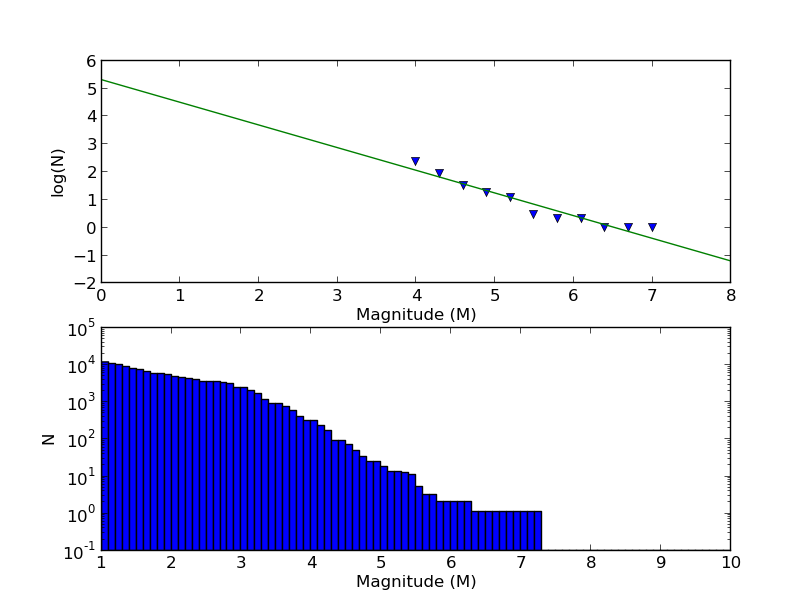
\includegraphics[width=0.6\linewidth,angle=0]{quake.png}
\caption{The output using all the data.}
\label{figure1}
\end{center}
\end{figure}





\subsection{Results}



\begin{figure}
\begin{center}
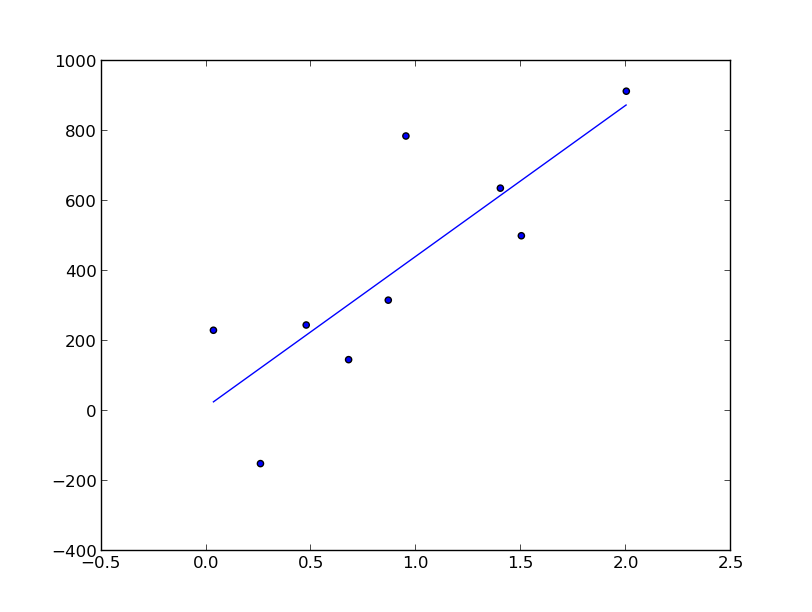
\includegraphics[width=0.6\linewidth,angle=0]{group.png}
\caption{The result using 9 groups data.}
\label{figure3}
\end{center}
\end{figure}

Using all the data, a=$-40.78 \pm 83.44$ Km/s and b=$454.16 \pm 75.24$ Km/s/Mpc, and the output plot is here ~\ref{figure2}

Using the 9 groups data, a=$11.21 \pm 126.59$ Km/s and b=$431.37 \pm 116.58$ Km/s/Mpc, and the output plot is here ~\ref{figure3} 

Since the age of the universe is 1/Hubble's constant \cite{hubblewiki} , I have the age of the universe is $215 \pm 36\times10^7 yrs$ for all data method and $227 \pm 61\times10^7 yrs$ for nine groups method.

\newpage
\section{Problem 2}
\subsection{Supernovae}
Find Hubble's constant from the intercept and slope output of the supernova program and compare with Hubble's value. Explain any discrepancies you observe.

\subsection{Numerical Analysis}
As with the supernovae, it no longer obeys the simple non-relativistic form of the Hubble's law:$v=rK+const$, the relativistic form must be employed:
$$
\mu=25+5log_{10}(\frac{cz}{H_o})+1.086(1-q_0)z+...
$$
Considering $q_0=0$ in our case, the equation can be written as:
$$
\mu=25+5log_{10}(\frac{c}{H_o})+5log_{10}z
$$
Therefore we can calculate the $H_o$ by means of the linear relationship between $\mu$ and $log_{10}z$,namely the intercept $I$and$H_o$can be linked by:
$$
I=25+5log_{10}(\frac{c}{H_o})
$$ 
So$H_o=\frac{c}{10^{{I/5}-5}}$

\subsection{result}

\begin{figure}
\begin{center}
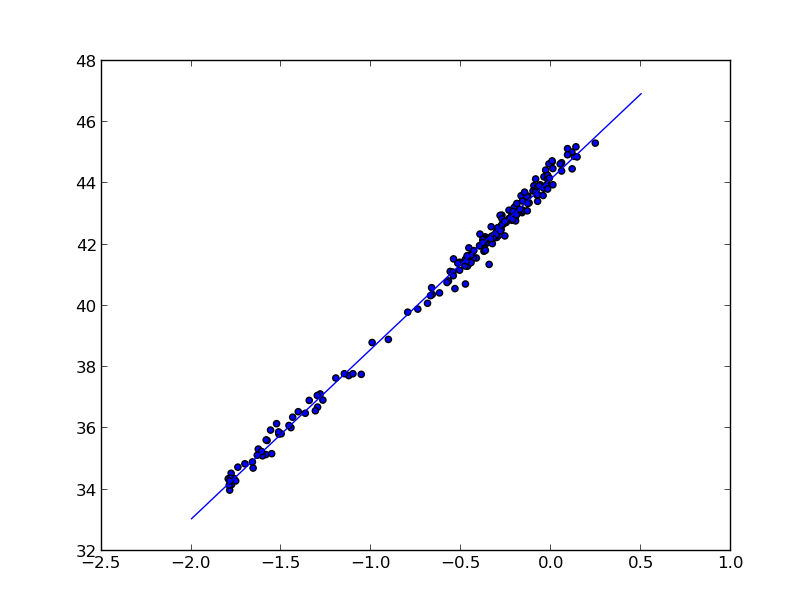
\includegraphics[width=0.6\linewidth,angle=0]{supernovaall.png}
\caption{The output using supernovae using all the data.}
\label{figure4}
\end{center}
\end{figure}

The linear fits result is shown in picture ~\ref{figure4}.
The slope is $5.553\pm0.026$ and the intercept is $44.152\pm0.022$
Correspondingly, the Hubble's constant is $H_o=44.329km/s/Mpc$

\newpage
\section{Problem 3}
\subsection{LOW AND HIGH RED SHIFT}
Divide the supernova data set into two subsets, low redshift and high redshift. Compute the slope separately for each of the two subsets. Can you conclude from your results that the expansion of the Universe is constant, accelerating, or decelerating?
\subsection{Numerical analysis} 
Based on z values we can divide data into two groups, one with z smaller than 0.7 and those larger than that.
To achieve that, I added some extra lines in the python script to write those two files.
\subsection{result}

\begin{figure}
\begin{center}
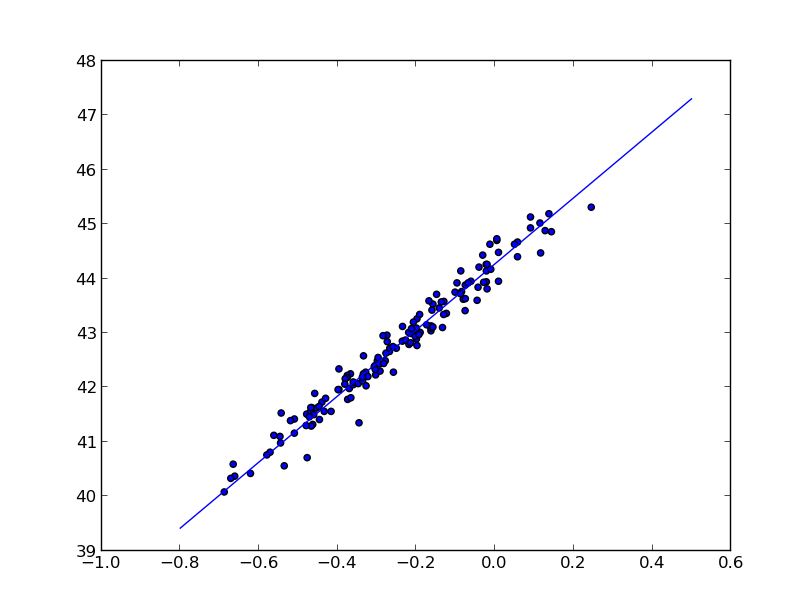
\includegraphics[width=0.6\linewidth,angle=0]{supernovagt7.png}
\caption{The output using supernovae using high shift the data.}
\label{figure5}
\end{center}
\end{figure}

\begin{figure}
\begin{center}
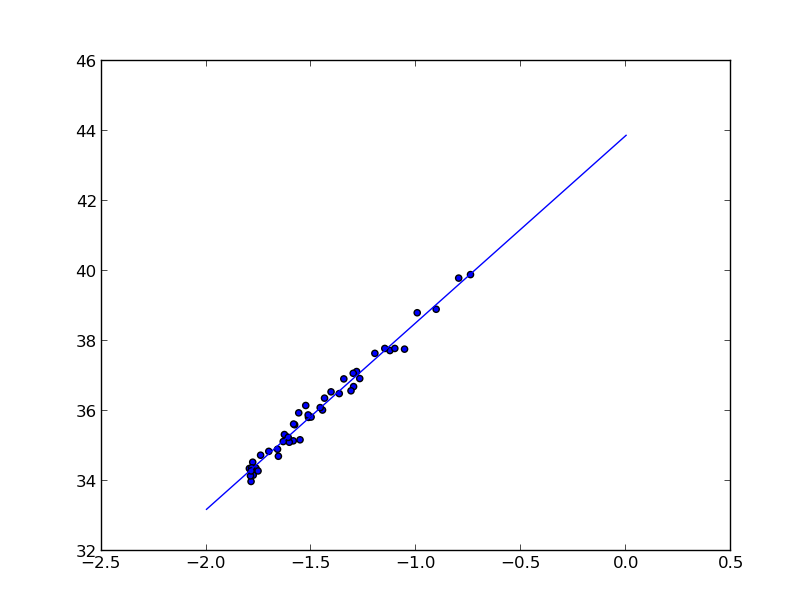
\includegraphics[width=0.6\linewidth,angle=0]{supernovast7.png}
\caption{The output using supernovae using low shift the data.}
\label{figure6}
\end{center}
\end{figure}

For the group with high shift~\ref{figure5}, we have The slope is $6.070\pm0.098$ and the intercept is $44.272\pm0.031$
Correspondingly, the Hubble's constant is $H_o=41.952km/s/Mpc$.

For the group with low shift~\ref{figure6}, we have The slope is $5.346\pm0.105$ and the intercept is $43.875\pm0.153$.
Correspondingly, the Hubble's constant is $H_o=50.363km/s/Mpc$.

Based on the result above, the expansion of the universe is increasing.


\newpage
\section*{Acknowledgements}

I discussed this assignment with my classmates and used material from the
cited references, but this writeup is my own.

\begin{thebibliography}{9}

\bibitem{The Physics of Earthquakes}
H. Kanamori and E.E. Brodsky, The Physics of Earthquakes, Physics Today 54, 34-40 (2001)\url{http://scitation.aip.org/content/aip/magazine/physicstoday/article/54/6/10.1063/1.1387590}

\bibitem{coursepage}
PHY 410-505 Webpage, \url{http://www.physics.buffalo.edu/phy410-505}.

\bibitem{Seismographs and Seismograms}
a brief introduction to seismographs and seismograms,\url{http://www.colorado.edu/physics/phys2900/homepages/Marianne.Hogan/graphs.html}.

\end{thebibliography}

\newpage
\appendix
\section{Appendix}

\subsection{python code}

The following python code was used to obtain the results in this report:

\lstinputlisting[language=python]{hubble_all.py}

\lstinputlisting[language=python]{supernovaall.py}

\end{document}
